\documentclass[12pt,twoside,openright,a4paper,english,brazil,sumario=tradicional]{abntex2}
\usepackage[utf8]{inputenc}
\usepackage[T1]{fontenc}
\usepackage{indentfirst}
\usepackage{color}
\usepackage{graphicx}
\usepackage{microtype}
\usepackage[brazilian,hyperpageref]{backref}
\usepackage[alf]{abntex2cite}
\usepackage{multicol}
\usepackage{multirow}
\usepackage{enumitem}
\usepackage{amsfonts}
\usepackage{amssymb}
\usepackage{listings}
\usepackage{tikz-uml}
\usepackage{uarial}
\renewcommand{\familydefault}{\sfdefault}
\usepackage{blindtext}
\graphicspath{{../images/}}
\renewcommand{\backrefpagesname}{Citado na(s) página(s):~}
\renewcommand{\backref}{}
\renewcommand*{\backrefalt}[4]{
   \ifcase #1 %
   Nenhuma citação no texto.%
   \or
   Citado na página #2.%
   \else		Citado #1 vezes nas páginas #2.%
   \fi}%

\titulo{Módulo de pré visualização para a ferramenta CGT - Ceará Game Tools}
\author{Joel Xavier Rocha\thanks{\texttt{joelxr@gmail.com}}}
\orientador{Prof. Dr. Carlos Hairon Ribeiro Gonçalves}
\local{Fortaleza}
\data{2015}
\instituicao{
   Instituto Federal de Ciência, Educação e Tecnologia do Ceará
   \par
   Engenharia de Computação}
\tipotrabalho{Monografia}
\preambulo{Trabalho de conclusão de curso apresentado à banca examinadora do Instituto Federal de Educação, Ciência e Tecnologia do Ceará para obtenção do grau de bacharel em Engenharia de Computação sob a orientação do Prof. Dr. Carlos Hairon Ribeiro Gonçalves.}
\definecolor{blue}{RGB}{41,5,195}
\makeatletter
\hypersetup{
   pdftitle={\@title},
   pdfauthor={\@author},
   pdfsubject={Trabalho de conclusão de curso},
   pdfcreator={pdfLaTeX},
   pdfkeywords={abnt}{latex}{abntex}{abntex2}{trabalho científico},
   colorlinks=true,
   linkcolor=blue,
   citecolor=blue,
   filecolor=magenta,
   urlcolor=blue,
   bookmarksdepth=4
}
\makeatother
\setlength{\parindent}{1.3cm}
\setlength{\parskip}{0.2cm}
\makeindex
\begin{document}
\selectlanguage{brazil}
\frenchspacing
\imprimircapa
\imprimirfolhaderosto*

% \begin{fichacatalografica}
%     \includepdf{fig_ficha_catalografica.pdf}
% \end{fichacatalografica}

% \includepdf{folhadeaprovacao_final.pdf}

\begin{agradecimentos}

\end{agradecimentos}
\setlength{\absparsep}{18pt}
\begin{resumo}
   O crescimento da industria de jogos em diversas áreas - como entretenimento e educação - torna necessário a elaboração de ferramentas que possibilitem a criação destes de forma simples, fácil e objetiva. Por esta razão, o projeto \emph{Ceará Game Tools} (CGT), tem como objetivo possibilitar isso aos usuários que não conhecem os meios e as técnicas envolvidas na criação de jogos.

   Então, é proposto nesse trabalho, melhorias importantes para a ferramenta CGT, principalmente, a pré visualização do jogo que está sendo construído e também dos seus objetos.
   \vspace{\onelineskip}
   \noindent
   \textbf{Palavras-chave}: CGT, ferramenta;
\end{resumo}
\pdfbookmark[0]{\listfigurename}{lof}
\listoffigures*
\cleardoublepage
\pdfbookmark[0]{\listtablename}{lot}
\listoftables*
\cleardoublepage
\pdfbookmark[0]{\contentsname}{toc}
\tableofcontents*
\cleardoublepage
\textual
\chapter{Introdução} % Ryllari
\label{chap:introducao}
% introduzindo sobre o que é o trabalho
Neste trabalho, é apresentado problemas existentes e pontos de melhorias na primeira versão da ferramenta de construção de jogos do projeto CGT (\texttt{ferramenta 1.0}). Bem como, de que modo essas questões foram tratadas e implementadas na segunda versão (\texttt{ferramenta 2.0}). A nova versão da ferramenta tem como objetivo melhorar o processe de criação de jogos e tornar essa tarefa mais intuitiva para o usuário final.
\section{O projeto CGT}
% Descrição/apresentação do projeto CGT
O projeto CGT que surgiu para tornar possível a qualquer pessoa a criação de jogos, assim como é explicado no trabalho \cite{monografia:aquino}, vem sido desenvolvido desde 2013 e possibilita a construção de jogos eletrônicos por qualquer pessoa, não sendo necessário conhecimentos em programação ou nas técnicas de criação de jogos. De foma fácil, simples e prática, a ferramenta, atende a necessidade da maior parte dos usuários, podendo produzir jogos de vários temas e para diversos fins, desde entretenimento a educação, por exemplo. Assim como, é proposto no \emph{web site} do projeto que explica, detalhadamente, o seu objetivo.
\begin{citacao}
   O projeto Ceará Game Tools tem como objetivo oferecer uma ferramenta para a construção de jogos. Em suma, qualquer um poderá criar seu próprio jogo utilizando componentes \emph{drag and drop} e os configurando. \cite{website:projeto-cgt}
\end{citacao}
\subsection{Vínculo com o CNPQ}
A idealização e o início do desenvolvimento da ferramenta CGT deu-se no ano de 2013, através do projeto Ceará Game Tools (CGT) – Pesquisa, Desenvolvimento e Comercialização de Games Temáticos da Cultura Cearense, que é uma inciativa do professor do IFCE Carlos Hairon Ribeiro Gonçalves  apoiado pelo CNPQ\footnote{Centro Nacional de desenvolvimento científico e tecnológico.} por meio do edital 80 de 2013 de número de processo 409227/2013-7.

A proposta deste projeto era desenvolver uma ferramenta de software livre para o desenvolvimento automático de \emph{games} casuais em que qualquer pessoa com conhecimentos medianos de operação de microcomputadores poderia desenvolver jogos. Neste caso, não há necessidade de codificação de software utilizando-se linguagens de programação, mas somente o desenvolvimento de modelos abstratos com o uso de aplicativos de software de uso livre. Além disso, ela pode gerar jogos que podem ser executados em vários sistemas operacionais(\emph{Windows}, \emph{Linux}, \emph{MacOS} e \emph{Android}). Desse modo, os desenvolvedores podem aferir retorno financeiro com a venda e/ou popularização dos jogos, democratizando este canal para todas as pessoas que queiram ingressar nessa área.
\subsection{Trabalhos anteriores}
A partir do projeto vinculado ao CNPQ, a primeira versão da ferramenta foi produzida, trabalhando o desenvolvimento dos jogos apenas com entrada e manipulação de dados, utilizando apenas botões e comandos, sem componentes \emph{drag and drop} ou módulo de pré-visualização. Com base no que foi desenvolvido ao longo desta etapa, foi produzido um trabalho acadêmico de conclusão de curso por título “Ceará Game Tools: Uma ferramenta de software livre para geração automática de games” \cite{monografia:aquino}.

Em aspectos gerais, esse trabalho apresenta todo o processo de criação da ferramenta Ceará Game Tools (CGT), que possui um ambiente de desenvolvimento visual simples e intuitivo e uma biblioteca de imagens e sons disponibilizados para os usuários desfrutarem. Além disso, nesse trabalho, relata trabalhos e \emph{softwares} similares ao CGT, descreve os métodos e ferramentas utilizados para o desenvolvimento da aplicação, além da forma com ela foi desenvolvida, os módulos em que o CGT está dividido, os pacotes e classes que compõem a ferramenta, seus diagramas, benefícios, bem como trabalhos futuros e possíveis melhorias para a ferramenta. Nesta última parte, o autor destaca a importância da criação de novas políticas que aumentem as opções dos jogos e implementem novas estruturas, do aumento no número de plataformas de exportação dos jogos desenvolvidos, além de adicionar módulo de pré-visualização do jogo, o qual se concentra o assunto do presente trabalho.

\subsection{Os módulos desenvolvidos para o projeto}
% ferramenta de construção de jogos
O projeto é composto por módulos que dividem entre si as funcionalidades existentes, esses módulos são mostrados e descritos na tabela \ref{table:modulos}. O módulo da ferramenta é o objeto de estudo para este trabalho e o objetivo deste módulo é implementar toda a interação com o usuário e ser responsável por apresentar o jogo a ele no momento da criação, tudo isso de forma intuitiva, simples e prática. Logo, pode-se notar que, esse módulo é essencial para o projeto e deve ser capaz de lidar com tudo que torna possível a criação de jogos.
\begin{table}[h]
   \centering
   \begin{tabular}{ | l | p{10cm} | }
      \hline
      \textbf{Módulos} & \textbf{Descrição} \\
      \hline
      \texttt{core} & Contém os objetos essenciais para o projeto. Assim como: Ator, Inimigo, Bônus. Na secção \ref{sec:objetos} pode ser visto todos os objetos. \\
      \hline
      \texttt{desktop} & Responsável por possibilitar a execução do jogo no computador, em ambientes que rodam os sistemas \emph{Windows}, \emph{Linux} e \emph{MacOS}. \\
      \hline
      \texttt{ferramenta} & Corresponde ao módulo objeto de estudo deste trabalho que possibilita a criação dos jogos. \\
      \hline
      \texttt{android} & Permite exportar o jogo para execução nos dispositivos que rodam o sistema operacional \emph{Android}. \\
      \hline
      \texttt{ios} & Permite exportar o jogo para execução nos dispositivos que rodam o sistema operacional \emph{iOS}. \\
      \hline
   \end{tabular}
   \caption{Módulos existentes no projeto CGT.}
   \label{table:modulos}
\end{table}
\section{Introdução ao problema}
\label{sec:intro-problema}
A identificação dos problemas e pontos de melhoria para a ferramenta foram percebidos, principalmente, Através do uso e estão relacionados a interação com o usuário final e como o jogo em produção é percebido.

A \texttt{ferramenta 1.0} é bastante robusta e atende o propósito de criar os objetos que compõem o jogo e, eventualmente, produzi-lo em forma de aplicação para a plataforma destino. Entretanto, a mesma carece em fornecer algum \emph{feedback} no momento da criação, obrigando ao usuário a sempre executar o jogo para poder perceber atributos essenciais dos objetos dele, tais como: a posição, o tamanho, a textura.

Por exemplo, sejam as posições de um novo objeto configuradas da forma que se deseja, logo após isso, naturalmente, o usuário executa o jogo para poder visualizar o que configurou, e também entender o que representa graficamente o número que inseriu. Pode-se ver esse processo ocorrendo na imagem \ref{fig:intro-problema-1}, as duas janelas que estão abertas são, respectivamente, a do jogo em execução e da ferramenta de criação. Portanto, podemos assumir que para todo objeto recém configurado, será preciso executar o jogo para ver o resultado da configuração. Ou seja, o processo de criação se torna bastante repetitivo.

\begin{figure}[h]
   \label{fig:intro-problema-1}
   \centering
   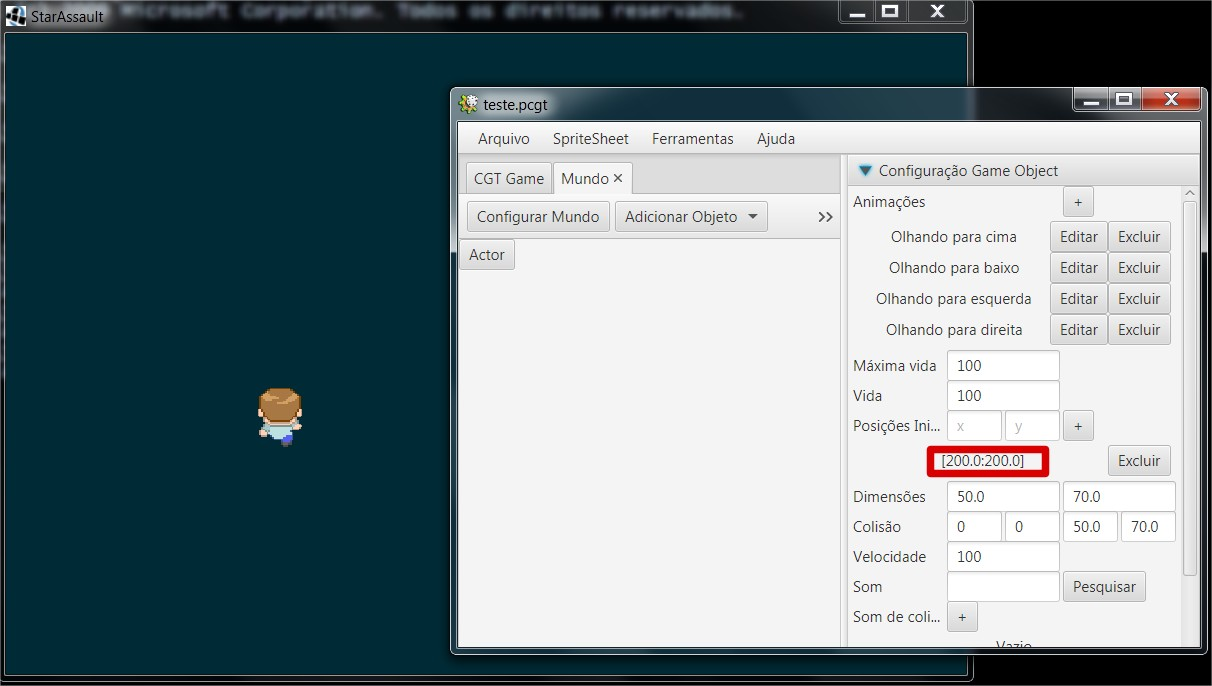
\includegraphics[width=0.7\textwidth]{images/problema-1.jpg}
   \caption{Problema de pré-visualização na \texttt{ferramenta 1.0}.}
\end{figure}

% mais problemas
Além disso, os controles que fazem parte da primeira versão da ferramenta, tornam, na maioria das vezes, oneroso o processo de configuração dos objetos. Por exemplo, na configuração das animações que possui um objeto é necessário criar as animações olhando no \emph{spritesheet}\footnote{Imagem que contém todas as faces de um objeto no jogo.} do objeto e preenchendo campos de texto com o valor da linha e coluna do \emph{sprite} correspondente a animação configurada (ver imagem \ref{fig:intro-problema-2}).

\begin{figure}[h]
   \label{fig:intro-problema-2}
   \centering
   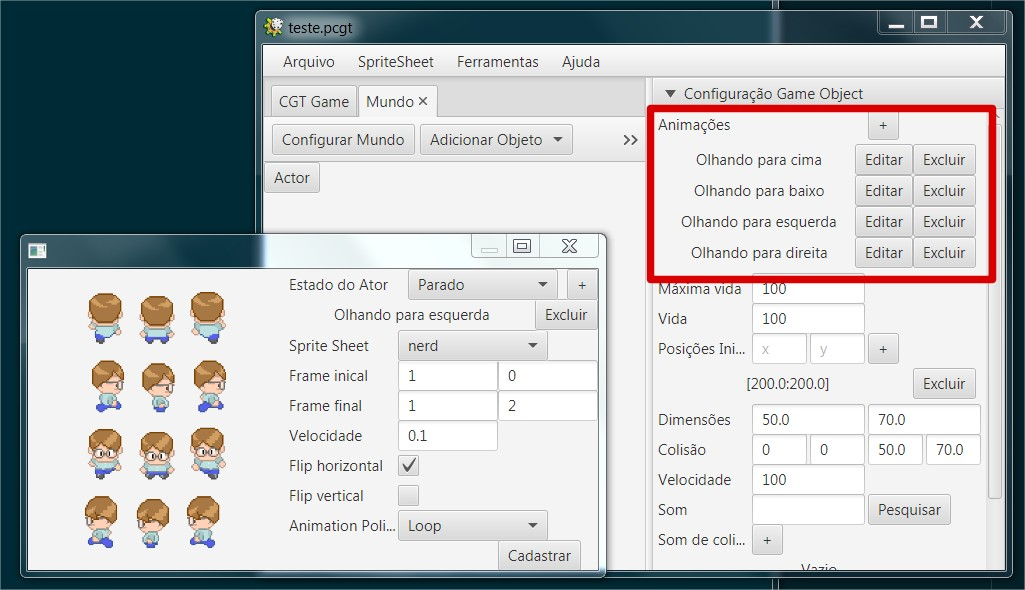
\includegraphics[width=0.7\textwidth]{images/problema-2.jpg}
   \caption{Problema com os controles na configuração de uma animação na \texttt{ferramenta 1.0}.}
\end{figure}

Os problemas encontrados na \texttt{ferramenta 1.0} foram a motivação para esse trabalho e serão descritos detalhadamente no capitulo \ref{chap:problemas}.

\section{Disposição do documento}
Este documento segue o método que consiste em: apresentar um problema, propor sua solução e, por fim, estudar as consequências da solução adotada. Dessa forma, tudo estará dividido basicamente nas três partes seguintes:
\begin{description}
   \item[Definição do problema] Mostrado no capítulo \ref{chap:problemas} que tem como objetivo enumerar detalhadamente os problemas e pontos de melhoria encontrados na \texttt{ferramenta 1.0} e como foram encontrados. Consequentemente, prepara-se uma lista das principais funcionalidades que farão parte da nova versão da ferramenta.
   \item[Proposta de melhorias] Corresponde ao capítulo \ref{chap:melhorias} que visa propor soluções para as questões encontradas anteriormente. Além disso, explicá-las e justificá-las detalhadamente, por fim demonstrando a solução adotada e como elas foram alcançadas.
   \item[Análise dos resultados] É um estudo de caso, mostrado no capítulo \ref{chap:caso}, com a nova versão da ferramenta, onde busca-se comparar o tempo de criação de jogo, a facilidade de uso e a quantidade de esforço necessário para configurar.
\end{description}

\chapter{Problema}
\label{chap:problemas}
% breve descrição do problema do preview
A ferramenta de construção de jogos do projeto CGT é robusta e atende aos objetivos propostos. Contudo, ela possui lacunas quando se trata da interação humano computador (IHC), onde é possível enumerar os seguintes pontos:

\begin{alineas}
\item A falta de pré-visualização dos objetos contidos no jogo dificulta a percepção do usuário, obrigando-o a sempre executar o jogo para observar as configurações que foram feitas;
\item Os controles não são claros e, assim, produzir um jogo pode acabar sendo uma experiência onerosa, confusa e repleta de configurações repetitivas.
\end{alineas}

A nova versão da ferramenta visa resolver os dois problemas mencionados, principalmente o primeiro item, por ser mais importante quando o assunto é usabilidade. Com isso em mente, faz-se necessário construir um jogo na primeira versão da ferramenta com o objetivo de perceber os problemas e as possíveis melhorias.

\section{Objetos de um jogo}
\label{sec:objetos}

Para enumerar todos os problemas e melhorias da \texttt{ferramenta 1.0}, é importante construir um jogo com ela e, para fazê-lo, é preciso conhecer os objetos que existem e como devemos configurá-los. Observar que, cada um deles possui suas características e configurações, assim como um propósito no jogo. A tabela \ref{table:objetos-desc} mostra os possíveis tipos objetos e a descrição deles.

\begin{table}[h]
\centering
\begin{tabular}{| l | p{7cm} |}
      \hline
      \textbf{Objeto} & \textbf{Descrição} \\
      \hline
      Mundo & Responsável por agregar todos os personagens de uma fase do jogo definindo o plano de fundo.  \\
      \hline
      Ator & Objeto controlado pelo jogador. \\
      \hline
      Inimigo & Objeto que causa dano ao ator e impede os objetivos dele. \\
      \hline
      Opositor & Objeto que impede ações do ator, que não pode ser ultrapassado e pode ser destruído pelo ator.  \\
      \hline
      Bônus & Objeto que promove bônus ao ator. \\
      \hline
      Projétil & Objeto que pode ser arremessado pelo ator. \\
      \hline
      Tela & Representa uma tela do jogo. \\
      \hline
      Botão de tela & Botão de uma tela do jogo. \\
      \hline
      Vida de um objeto & Representado através de uma barra, mostra a quantidade de vida que um objeto possui. \\
      \hline
      Munição de um objeto & A quantidade de projéteis que o ator ainda pode arremessar. \\
      \hline
   \end{tabular}
\caption{Objetos que existem em um jogo.}
\label{table:objetos-desc}
\end{table}

Notar que, eles são inseridos na ferramenta a medida que o usuário ver necessidade e são responsáveis por dar liberdade ao autor de construir vários formatos de jogos, por exemplo jogos de: perguntas e respostas, concluir percurso, derrotar inimigo, sobreviver determinado tempo.

A seguir, mostra-se um jogo de exemplo na ferramenta e, com isso, os problemas e pontos de melhoria, notar que, o manual da ferramenta está na parte de anexos e pode ser consultado para entender como funciona a criação de cada um dos objetos citados.

\section{Dificuldades encontradas}
\label{sec:dificuldades}
% detalhar dificuldades com figuras da ferramenta 1.0, fazer um jogo de exemplo que será usado posteriormente
As dificuldades encontradas na ferramenta foram relacionadas de acordo com a compreensão de cada componente existente nela, chama-se dificuldade qualquer empecilho na ferramenta que dificulte a criação e configuração de algum objeto ou o entendimento do papel dele no jogo. Assim, é percebido uma dificuldade e então ela é enumerado como problema encontrado. As seções seguintes trazem cada um dessas dificuldades encontradas.

Notar que, a \texttt{ferramenta 1.0} está disponível no \href{http://www.cgt.ifce.edu.br/downloads.php}{site do projeto CGT} na secção de \emph{downloads}\footnote{http://www.cgt.ifce.edu.br/downloads.php}.

\subsection{Organização dos objetos}
Um dos pontos mais importantes quando se trata de criação de jogos, é que - no decorrer do desenvolvimento - eles podem se tornar enormes e, para a ferramenta, um jogo é um conjunto de objetos e suas respectivas propriedades. Logo, é imprescindível que os objetos possam ser vistos de forma lógica e, mais importante, organizada, já que, assim, serão acessados facilmente, pois o usuário terá necessidade de retornar a eles para melhorar ou corrigir alguma configuração.

Além disso, vale ressaltar que entre os objetos existe uma relação de pertinência, um ator está inserido em um mundo, assim como o inimigo que ele precisa derrotar, essa hierarquia precisa ser levada em consideração na ferramenta e o jogo será criado respeitando essas relações.

Na figura \ref{fig:objetos_disp}, pode-se visualizar um jogo sendo criado e - a partir dessa imagem - pode-se notar que a ferramenta é dividida em cinco áreas importantes que estão descritas na tabela \ref{table:ferramenta_areas}. Os botões que representam objetos são organizados por colunas que representam as categorias: ator, inimigos, opositores, bonificações e informações da tela. A medida que é adicionado um novo objeto para a aba, este é posicionado na coluna correta.

Essa forma de organizar os objetos do jogo possui a vantagem de ser objetiva quanto a exibir apenas o conteúdo que importa para aquele agregador (uma fase do jogo ou uma tela). No entanto, a medida que o usuário vai inserindo elementos ao jogo, essa visão - embora organizada - pode perder o significado, isto é, precisa-se de algo além de um botão com um nome gerado automaticamente para representar um objeto. Como pode ser percebido na figura \ref{fig:objetos_disp}, nesse jogo, existem quatro inimigos configurados, mas não se sabe quais são as características deles apenas olhando para os botões, ou seja, o usuário precisa selecionar um a um até encontrar qual deles é o que ele procura. Sendo assim, a ação de reconfigurar um objeto pode tornar-se difícil a medida que novos itens forem sendo adicionados ao jogo.

\begin{table}[h]
   \centering
   \begin{tabular}{| l | p{8cm} |}
      \hline
      \textbf{Menu} & No menu é possível realizar ações que refletem no projeto todo, por exemplo: salvar, adicionar \emph{spritesheet}, executar o jogo. \\
      \hline
      \textbf{Abas} & As abas representam os agregadores de objetos, podem conter a aba inicial do projeto, um \emph{mundo} ou uma tela. \\
      \hline
      \textbf{\emph{Toolbar}} & Permite realizar ações referentes ao agregador, se for de um mundo possibilitar adicionar um inimigo ao jogo, por exemplo. \\
      \hline
      \textbf{Botões de objetos} & Cada objeto é representado por um botão que pertencem a uma determinada aba. \\
      \hline
      \textbf{Painel lateral} & Mostra as configurações do objeto selecionado, ao clicar em qualquer botão será mostrado as configurações daquele objeto.  \\
      \hline
   \end{tabular}
   \caption{Controles utilizados na primeira versão da ferramenta.}
   \label{table:ferramenta_areas}
\end{table}

\begin{figure}[h]
\label{fig:objetos_disp}
\centering
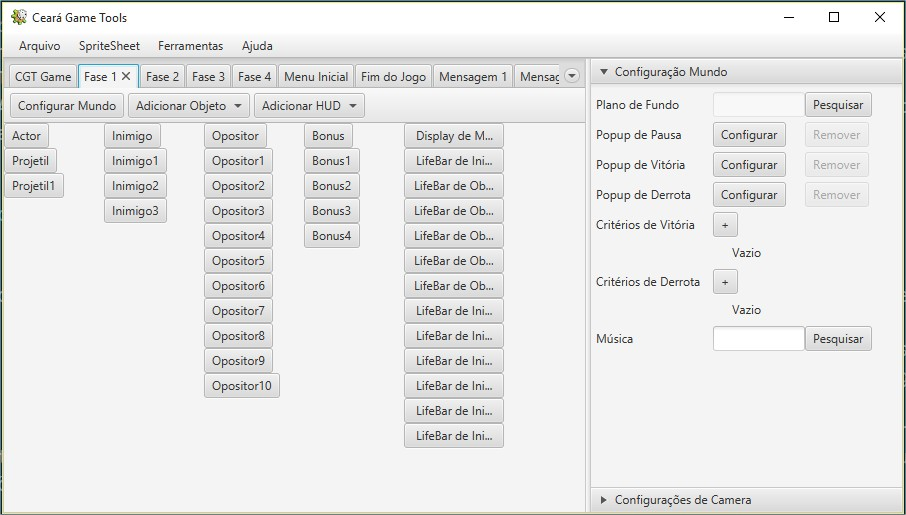
\includegraphics[width=0.8\textwidth]{images/objetos_disposicao.jpg}
\caption{Disposição dos objetos na versão anterior da ferramenta.}
\end{figure}

\subsection{Painéis de configuração dos objetos}

Todos os itens que fazem parte de um jogo possuem características que os definem, sendo assim cabe a ferramenta prover ao usuário final uma forma clara e objetiva de configurá-las. Além disso, a ferramenta tem obrigação de validar os dados e guiar o usuário nos casos mais complexos, assim como dar um significado para o dado que está sendo recebido. Por exemplo, vamos supor que exista um objeto recém adicionado no jogo e que pretendemos configurar a sua posição inicial na tela, a ferramenta recebe essa configuração através de dois números que são, respectivamente, as posições cartesianas $x$ e $y$ do objeto, deve-se verificar se essas posições estão contidas no retângulo que representa a tela do jogo, assim como fornecer ao usuário formas de saber o que significa o valor que ele está configurando.

\begin{figure}[h]
   \label{fig:obj_pos_inicial}
\centering
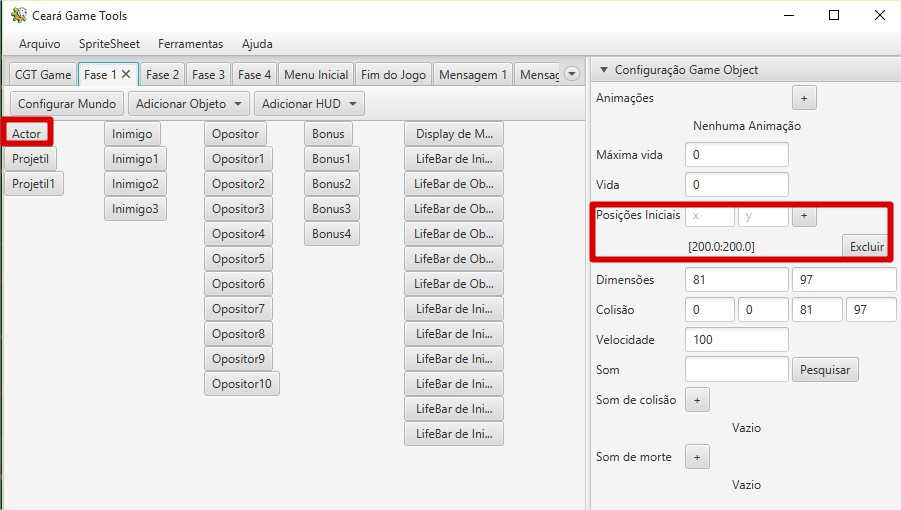
\includegraphics[width=0.8\textwidth]{images/pos_inicial.jpg}
\caption{Configuração da posição inicial de um objeto na primeira versão da ferramenta.}
\end{figure}

\begin{figure}[h]
   \label{fig:obj_dimensoes}
\centering
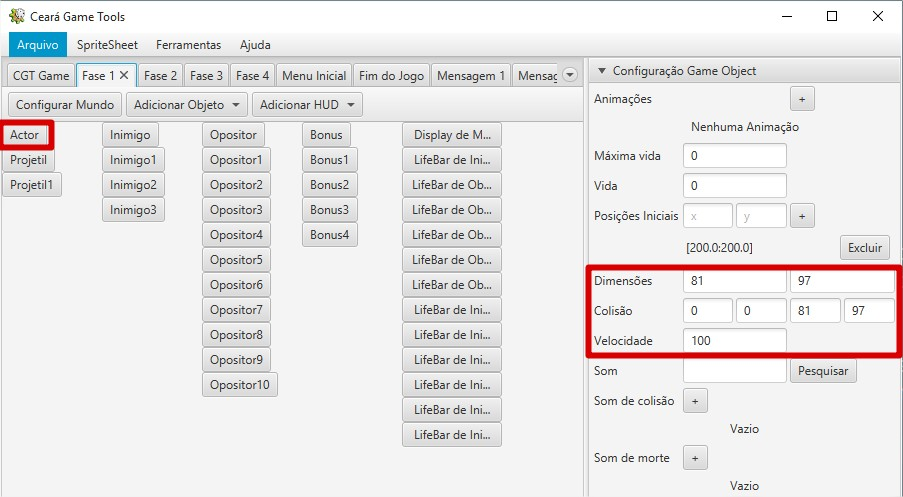
\includegraphics[width=0.8\textwidth]{images/obj_dimensoes.jpg}
\caption{Configuração das dimensões de um objeto na primeira versão da ferramenta.}
\end{figure}

\subsection{Pré visualização dos objetos}

Os principais problema dos painéis de configuração da \texttt{ferramenta 1.0} estão diretamente relacionados a falta de pré-visualização dos objetos, já que não há forma melhor que a pré-visualização quando se trata de perceber o significado de uma configuração feita.


\section{Game JAM} % Ryllari

\chapter{Descrição das melhorias} % Joel
\label{chap:melhorias}
\section{Pontos de melhoria}
\section{Detalhes da implementação do novo módulo}
\subsection{Métodos e ferramentas}
\subsection{Descrição do módulo}

\chapter{Estudo de caso}
\label{chap:caso}
\section{Análise dos resultados}
\section{Comparativo}
\section{Jogo exemplo}
\section{Projeto de extensão}

\chapter{Conclusão e trabalhos futuros}
\label{chap:conclcsao}

\postextual
\bibliography{references}

\begin{apendicesenv}
   \partapendices
   \chapter{Diagramas UML}
   \label{chap:diagramas}

   \section{Diagrama de classes}
   No diagrama de classes a seguir, temos a notação UML para as classes do módulo \texttt{ferramenta} do projeto CGT que estão localizadas dentro do pacote \texttt{br.edu.ifce.cgt.application}.

   \begin{figure}[h]
      \label{fig:diagrama-classes}
      \centering
      \begin{tikzpicture}
         \begin{umlpackage}{vo}
            \umlinterface{DrawableObject}{}
            {
               getObject() : T \\
               setObject(obj : T) : void \\
               getPane() : Node \\
               drawObject() : void \\
               drawConfigurationPanel() : void \\
               onCreate() : void \\
               onStart() : void \\
               destroy() : boolean }
            \umlclass[x=8,y=0]{AbstractDrawableObject}
            {
               - object : T \\
               - drawableObjectPane : Pane \\
               - drawConfigurationPanel : Pane
            }
            {
               getDrawableObjectPane() : Pane \\
               getDrawableConfigurationsPane() : Pane \\
               updateDrawPane(node : Node) : void \\
               updateConfigPane(node : Node) : void \\
               updateConfigPane(pane : Pane) : void
            }
            \umlclass[x=0,y=-6]{CGTProjectDrawable}
            {
               - size : Rectangle \\
               - projectPane : ConfigProjectPane
            }{}
            \umlclass[x=8,y=-6]{CGTGameObjectDrawable}
            {
               - gameObjectTitledPane : GameObjectPane \\
               - worldName : String \\
               - bounds : Rectangle \\
               - collision : Rectangle \\
               - preview : Draggable
            }
            {}
            \umlclass[x=0,y=-9]{CGTGameActorDrawable}{}{}
            \umlclass[x=8,y=-10]{CGTGameEnemyDrawable}{}{}
            \umlclass[x=0,y=-11]{CGTGameOppositeDrawable}{}{}
            \umlclass[x=8,y=-12]{CGTGameBonusDrawable}{}{}
            \umlclass[x=0,y=-13]{CGTGameProjectitleDrawable}{}{}
            \umlclass[x=8,y=-14]{CGTGameScreenDrawable}{}{}
            \umlclass[x=0,y=-15]{CGTButtonScreenPreview}{}{}
            \umlclass[x=8,y=-16]{CGTLifeBarDrawable}{}{}
            \umlclass[x=0,y=-17]{HUDComponetDrawable}{}{}
            \umlclass[x=8,y=-18]{DrawableObjectTreeCellImpl}{}{}
            %\umlimpl{DrawableObject}{AbstractDrawableObject}
            %\umlimpl{AbstractDrawableObject}{CGTProjectDrawable}
            %\umlimpl{AbstractDrawableObject}{CGTGameObjectDrawable}
            %\umlimpl{CGTGameObjectDrawable}{CGTGameActorDrawable}
            %\umlimpl{CGTGameObjectDrawable}{CGTGameEnemyDrawable}
            %\umlimpl{CGTGameObjectDrawable}{CGTGameOppositeDrawable}
            %\umlimpl{CGTGameObjectDrawable}{CGTGameBonusDrawable}
            %\umlimpl{CGTGameObjectDrawable}{CGTGameProjectitleDrawable}
         \end{umlpackage}
      \end{tikzpicture}
      \caption{Diagrama de classes UML para o módulo implementado.}
   \end{figure}

\end{apendicesenv}

\begin{anexosenv}
   \partanexos
   \chapter{Manual da ferramenta}

   \chapter{Código fonte}
\end{anexosenv}
\phantompart
\printindex
\end{document}
